% Drawing 85/01-1 -- folder 85, batch 01, archive page 5 (PDF page 6).
% Transcription: dans la marge gauche, un petit croquis : deux droites se coupant, une troisième demi-droite issue de leur point commun, l'angle $\theta_i$ marqué entre les deux premières, et un arc fléché marqué $\rho_i$ allant de la première à la troisième (la rotation)
% Kind: two lines, an angle theta_i and an arrowed arc rho_i. Method 2 (schematic redraw from the facsimile). Status: ok.
% Notes: Ink. Two lines through one computed point (the steep one heavier at its lower end) and a third stroke from that point to the upper right; the small arc and theta_i between the lower ray of the steep line and the second line; the arrowed arc rho_i from the lower ray of the steep line up to the third stroke. The transcription's note has two lines only; the third stroke, where the arc ends, is on the page. Redrawn 2026-11-12 (issue 128): to check again.
% Coordinates: 1 unit = 1 mm = 1/100 of the crop width (bbox in page fractions: [0.1, 0.59, 0.3, 0.7]).
% Redrawn by Claude (claude-fable-5-2), issue #128, 2026-11-12; not checked by a human; not compiled (no TeX in the session).
% Rights: reproduces part of the work -- behind RENDER_TRANSCRIPTS, never published by itself.
\documentclass[tikz,border=3pt]{standalone}
\usepackage{amsmath,amssymb}
\usetikzlibrary{patterns,arrows.meta}
\tikzset{pencil/.style={black!45}, struck/.style={black!35}, mpt/.style={circle,draw,inner sep=1.3pt}, pt/.style={circle,fill,inner sep=0.9pt}, opt/.style={circle,draw,fill=white,inner sep=1.1pt}}
\begin{document}
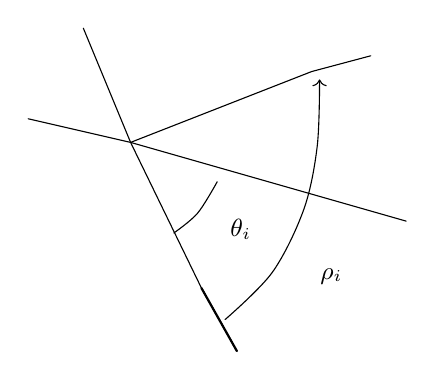
\begin{tikzpicture}[x=1mm,y=1mm,line cap=round,line join=round,font=\scriptsize]
\draw (18,-15) -- (24,-29.5) -- (33,-48) -- (37.5,-56);
\draw[thick] (33,-48) -- (37.5,-56);
\draw (11,-26.5) -- (24,-29.5) -- (59,-39.5);
\draw (24,-29.5) -- (47,-20.5) -- (54.5,-18.5);
\draw[->] plot[smooth, tension=0.55] coordinates {(36,-52) (42,-46) (46,-38) (47.7,-30) (48,-21.5)};
\draw plot[smooth, tension=0.55] coordinates {(29.5,-41) (32.5,-38.5) (35,-34.5)};
\node[inner sep=1pt] at (38,-40.5) {\small $\theta_i$};
\node[inner sep=1pt] at (49.5,-46.5) {\small $\rho_i$};
\end{tikzpicture}
\end{document}
